%!TEX root = ../thesis.tex
In this section we are going to cover our evaluation of our \emph{textile touch} explorative prototype, more specifically this is the latest prototype covered in \ref{ch:textiletouch:it3}~(\nameref{ch:textiletouch:it3}).
We have two primary goals of this evaluation.
On the one hand, we want to evaluate on the interaction potentials of using simple gestures as input control.
This goal involves using the prototype as an interactive device to control existing devices of the home.
On the other hand, we want to explore our prototype in alternative contexts.
This goal should shed light on the prototype's potential of encouraging alternative usages than controlling existing devices.
Evaluations were done over three rounds to get feedback from a diverse set of people, both technical and non-technical.
\blank
As mentioned earlier in \emph{ \nameref{ch:textiletouch:it3} } we have developed a simple audio and video application which mimics some of the functionality of a television and a stereo system.
This application was used as the starting point for evaluating the value of using the prototype for controlling existing devices.
During the evaluation we would connect the prototype setup and laptop to the home TV to resemble the real situation.
The prototype would then for instance be laid as part of the sofa, as a table cloth or attached to a wall as for example wallpaper.
From there on the basics of interaction were understood and further discussions and explorations could be made extending beyond the limits of the audio/video application.

Moving on from looking at the potentials of controlling existing devices of the home, the evaluations would take a more discussion-oriented direction where alternative usages and activities were the primary focus.
Ideas were brainstormed in plenum while we occasionally would pitch a few of our own ideas for potential usages.
\blank
An overall note to be taken from the evaluations was that the participants found it intriguing to try out the prototype.
Not so much for the purpose of the simple test application, but more for the idea of interacting with textile and using it for digital input.
Surely they are accustomed to using touch interaction on the small surfaces of everyday consumer devices such as displays and touchpads, but not with inherently non-electronic materials such as textile.
\blank
In the next section we will evaluate on the performance of our prototype and then continue with the conceptual potentials in the subsequent two sections.

\subsection{Performance and interaction feedback}

In this section we will discuss the prototype concerning performance and feedback and some of the improvements suggested during evaluations.

% refresh rate
The limitations of the refresh rate of the hardware were noticed by all participants.
The consequence was that they had to perform touch input in a more careful manner and with slower motions than they wanted to.
The participants' touch strokes were in general much faster than anticipated, which is likely due to us having done much of our testing during development and therefore have been more careful.
They were all able to adapt to it and perform their intended actions with success, but it did of course put a constraint on the interaction.

% softness
In our first evaluation we tested a scenario with a sofa with textile touch embedded.
The softness of the sofa made touch input readings inconsistent and unstable.
The reason for this was that the prototype was not part of the sofa construction which makes even small movements and pressure inputs push the prototype around on the surface of the sofa.
This makes the pattern constituting a touch look different than when used on a hard surface which we have not taken into account in our software.
We quickly fixed this by laying a thin plastic cutting board underneath the prototype which made sure pressure propagations were correct again.

% fb: vibrations
The idea of a pulsating vibration during touch was well received as an indication of touch being recorded and as indication of the boundary between the interactive area and the non-interactive area.
As we anticipated, the quality of the haptic feedback got some critique and it was pointed out that it should give a stronger sensation.
We had placed the vibration motor in the center beneath the prototype and vibrations were therefore only noticeable in that area.
With a less powerful motor, like ours, the subtle touch sensation of ones hand against the texture of the linen could easily drown the vibrations as well.

% fb: visual on display
A concern brought up by several participants was that there was a lack of indication of the stroke one had just applied.
A promising visual feedback technique for display-oriented interaction was suggested by one of the participants.
The idea was to get real-time feedback on a display when providing touch input by seeing the strokes being made as an overlay on the display.
The strokes would then quickly fade away again to not obstruct the viewing experience. 
In figure~\ref{fig:textiletouch:eval:overlay} we have made an illustration of two semi-transparent strokes overlaying a TV programme as example. 

\begin{figure}[h]
  \centering
  \begin{subfigure}[t]{.44\textwidth}
    \centering
    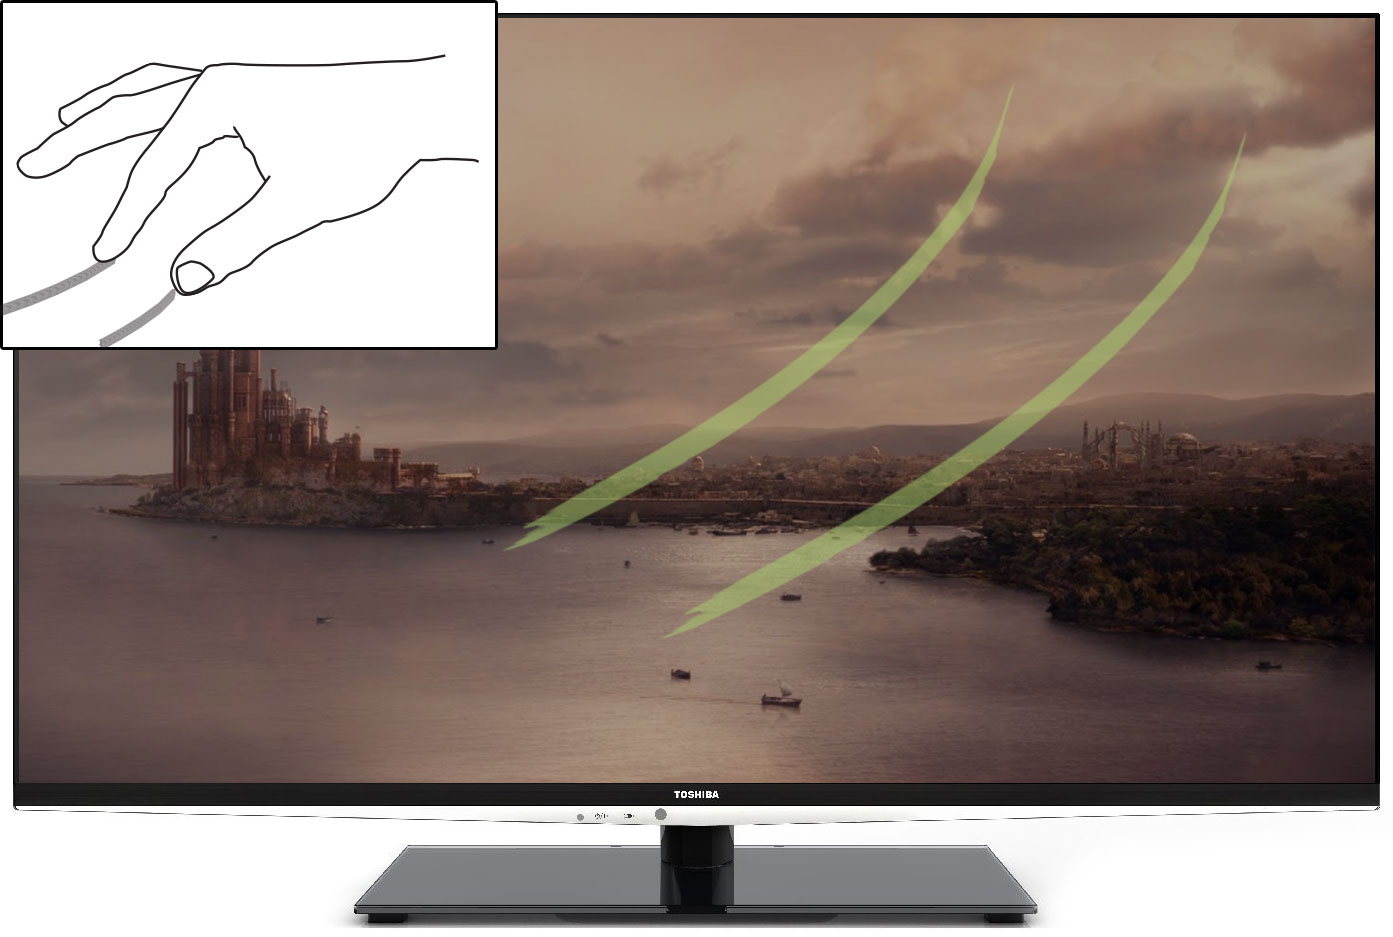
\includegraphics[width=\linewidth]{figures/touch/evaluation/gesture_overlay}
    \caption{The real-time overlay during touch. This ascending or descending two stroke gesture could for instance mean `volume up' or `down'.}
  \end{subfigure}%
  \hspace{0.02\textwidth}
  \begin{subfigure}[t]{.44\textwidth}
    \centering
    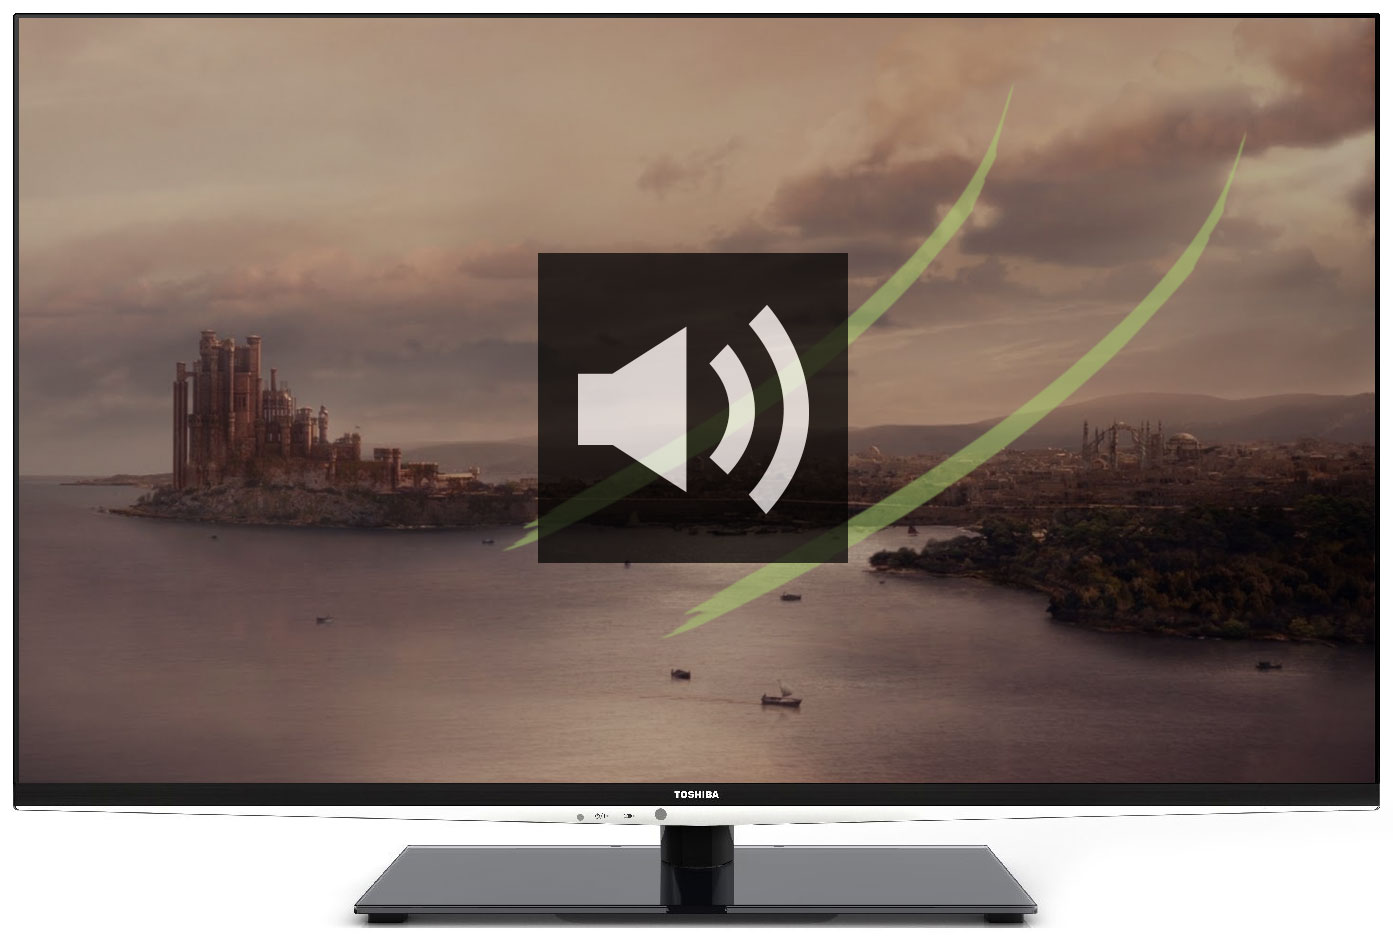
\includegraphics[width=\linewidth]{figures/touch/evaluation/gesture_overlay_2}
    \caption{The indication that a `volume' action was performed.}
  \end{subfigure}
  \caption{Gesture input as an overlay for real-time feedback.}
  \label{fig:textiletouch:eval:overlay}
\end{figure}

% fb: visual through LEDS
This visual feedback technique could be very convenient when actions are directed towards a device with a digital display, but not possible in a display-less context.
The single LED we installed beneath the prototype did not prove to be very useful by itself, but its ability to shine through the linen did show potential.
We discussed a larger deployment where a low resolution grid of tiny LEDs could be embedded beneath the textile surface and follow movements by illuminating at touch points and get a direct visual feedback (see figure~\ref{fig:textiletouch:eval:backlighting}).
This approach is again limited to applications where the surface material allows for illumination to shine through, but it does extend beyond textile materials.

\begin{figure}[h]
  \centering
  \begin{minipage}[b]{.8\textwidth}
    \centering
    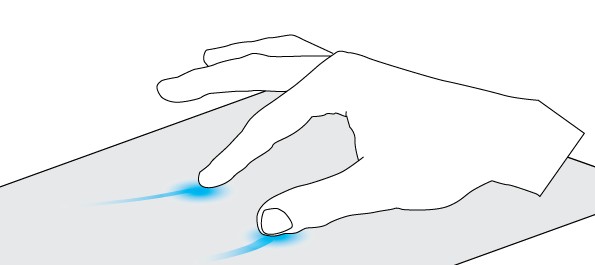
\includegraphics[width=.7\linewidth]{figures/touch/evaluation/backlid_textile}
  \caption[Illumination directly beneath touch points.]
  {Illumination directly beneath touch points.}
  \label{fig:textiletouch:eval:backlighting}
  \end{minipage}
\end{figure}

\subsection{The prototype as a controller for existing devices}

Several participants pointed out the ``coolness'' of being able to control devices in the environment without having to find the appropriate remote control or having to approach the specific device.
Most participants were quick to come up with their own examples of what could be controlled by the prototype, as their imagination was spurred by the novel interaction surface.
For example, being able to control the curtains or the radiator for heating adjustments from ones current position by using the nearest touch sensitive surface.
We interpret this creativity as being due to the open-ended nature of the prototype.
Figure~\ref{fig:textiletouch:eval:kaia-gitte-troels} contains a selection of photos from an initial small test-evaluation at the office with some friends.

\begin{figure}[t]
        \centering
        \begin{subfigure}[b]{0.44\textwidth}
                \centering
                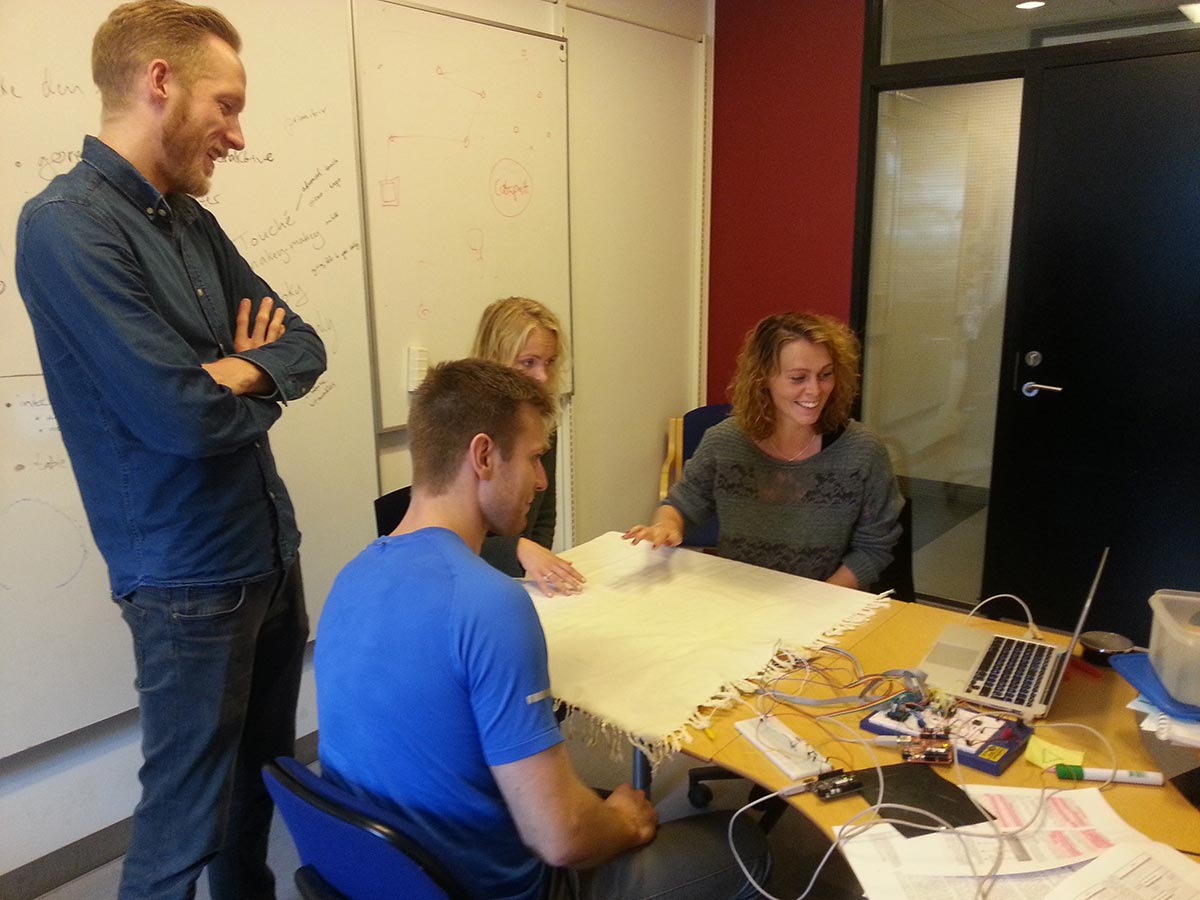
\includegraphics[width=\textwidth]{figures/touch/evaluation/kaia-gitte-troels/alle}
                \label{fig:textiletouch:eval:kaia-gitte-troels:alle}
        \end{subfigure}%
        \hspace{0.02\textwidth}
        \begin{subfigure}[b]{0.44\textwidth}
                \centering
                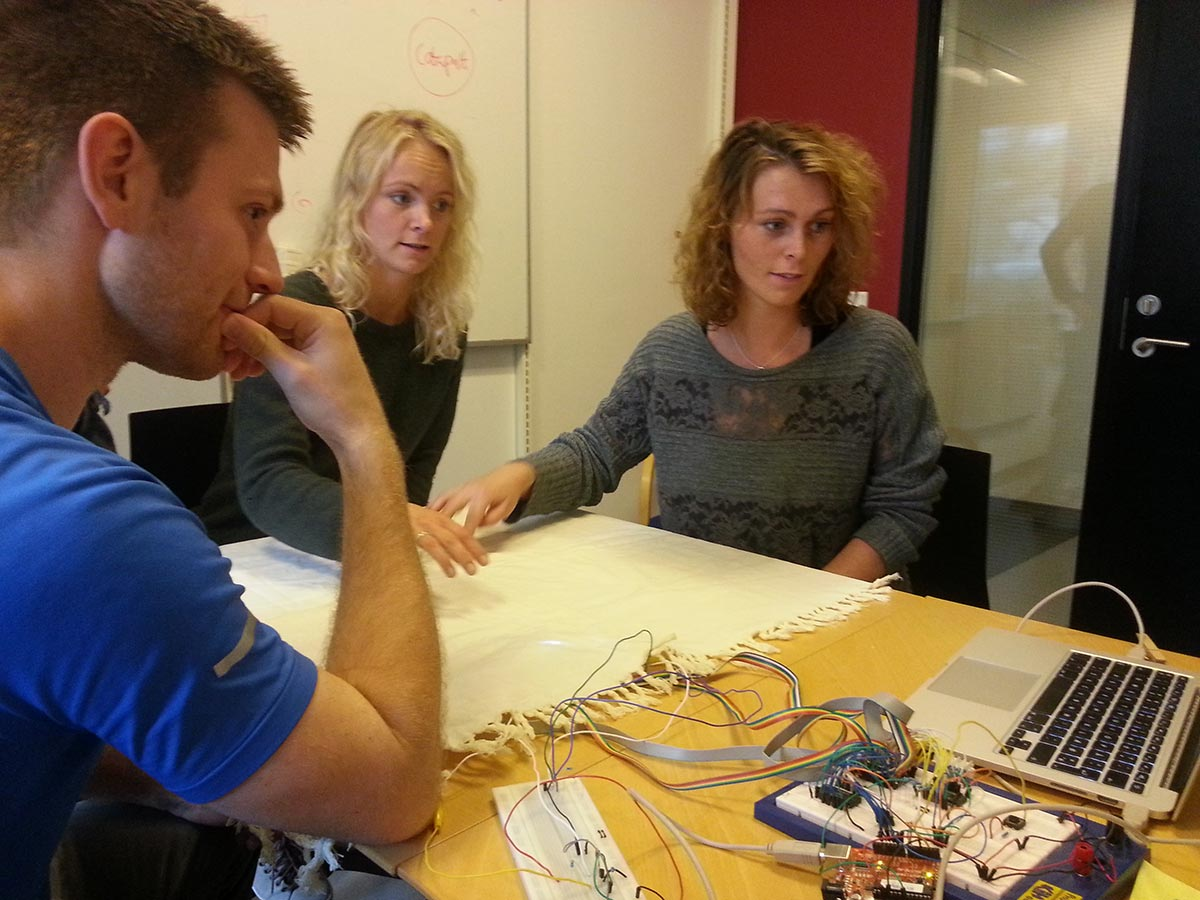
\includegraphics[width=\textwidth]{figures/touch/evaluation/kaia-gitte-troels/kaia-gitte2}
                \label{fig:textiletouch:eval:kaia-gitte-troels:kaia-gitte2}
        \end{subfigure}

        \begin{subfigure}[b]{0.9\textwidth}
                \centering
                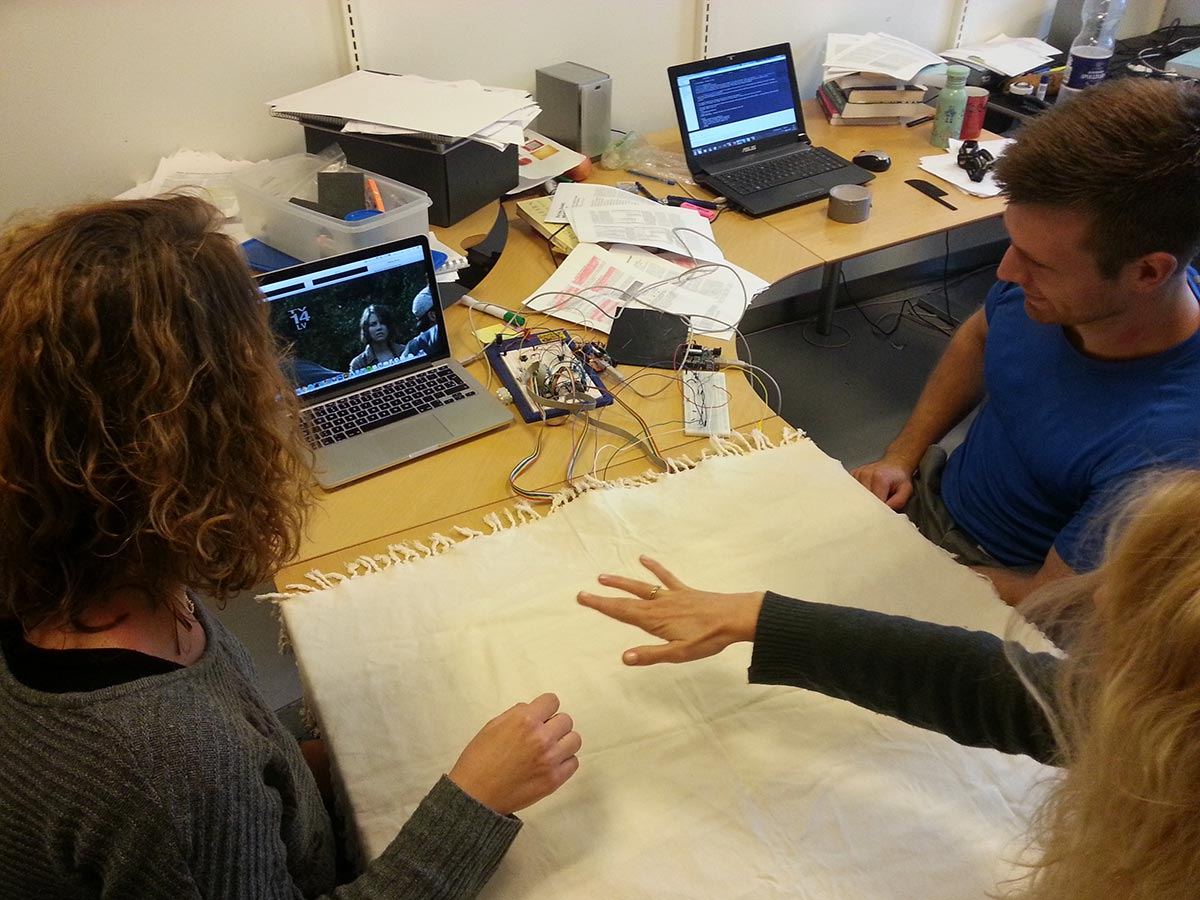
\includegraphics[width=\textwidth]{figures/touch/evaluation/kaia-gitte-troels/kaia-gitte}
                \caption{The prototype and audio/video applications is being tested.}
                \label{fig:textiletouch:eval:kaia-gitte-troels:kaia-gitte}
        \end{subfigure}
        \caption{An initial evaluation at the office.}
        \label{fig:textiletouch:eval:kaia-gitte-troels}
\end{figure}

Our teenager participant was quite eager to try out the prototype.
He had an intuitive understanding of the interaction and went about exploring the possibilities as soon as he sat down with it.
This resulted in him finding and making sense of some of the gesture-mappings without us instructing him beforehand, such as ``if this means volume up, this must be down \dots''.
Figure~\ref{fig:textiletouch:eval:sebastian} contains a selection of photos from the evaluation with him.
He was also fond of trying alternative ways of creating touch input, for example by moving the prototype to the floor and using his feet, see figure~\ref{fig:textiletouch:eval:sebastian:feet}.
This was however mostly for the fun of it.

\begin{figure}[t]
    \centering
    \begin{subfigure}[t]{0.44\textwidth}
        \centering
        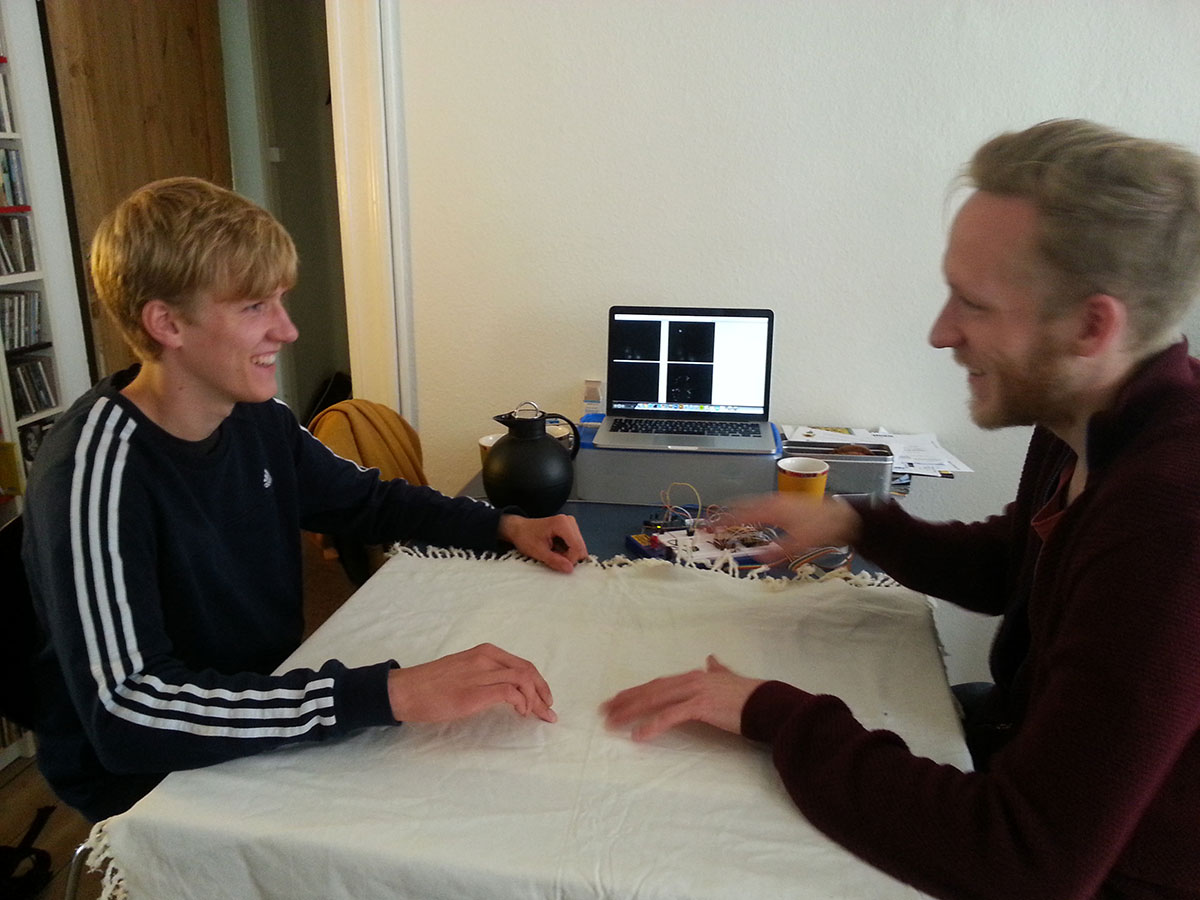
\includegraphics[width=\textwidth]{figures/touch/evaluation/sebastian/table}
        \caption{Using the prototype as a tablecloth.}
        \label{fig:textiletouch:eval:sebastian:table}
    \end{subfigure}%
    \hspace{0.02\textwidth}
    \begin{subfigure}[t]{0.44\textwidth}
        \centering
        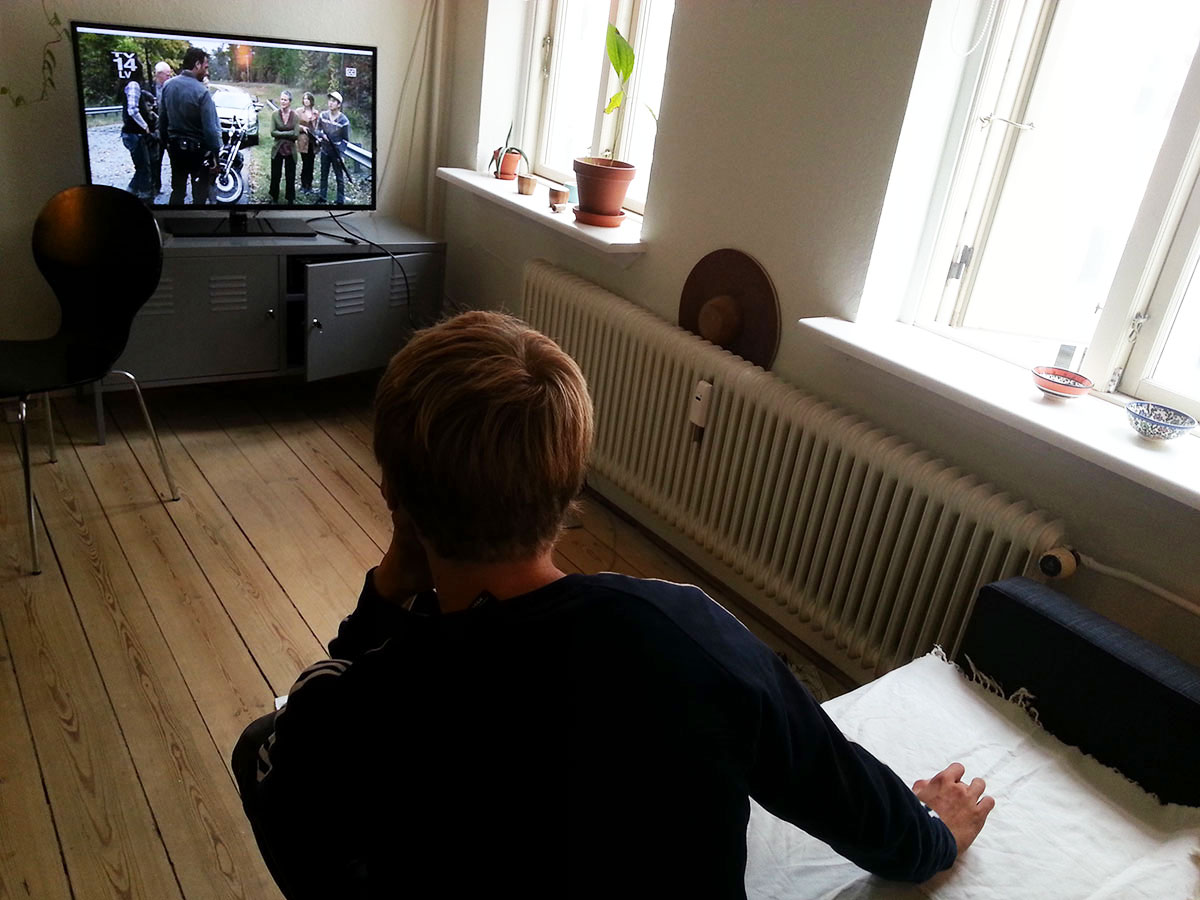
\includegraphics[width=\textwidth]{figures/touch/evaluation/sebastian/sofa_behind_seb}
        \caption{Teenager controlling the video application.}
        \label{fig:textiletouch:eval:sebastian:sofa_behind}
    \end{subfigure}

    \begin{subfigure}[t]{0.44\textwidth}
        \centering
        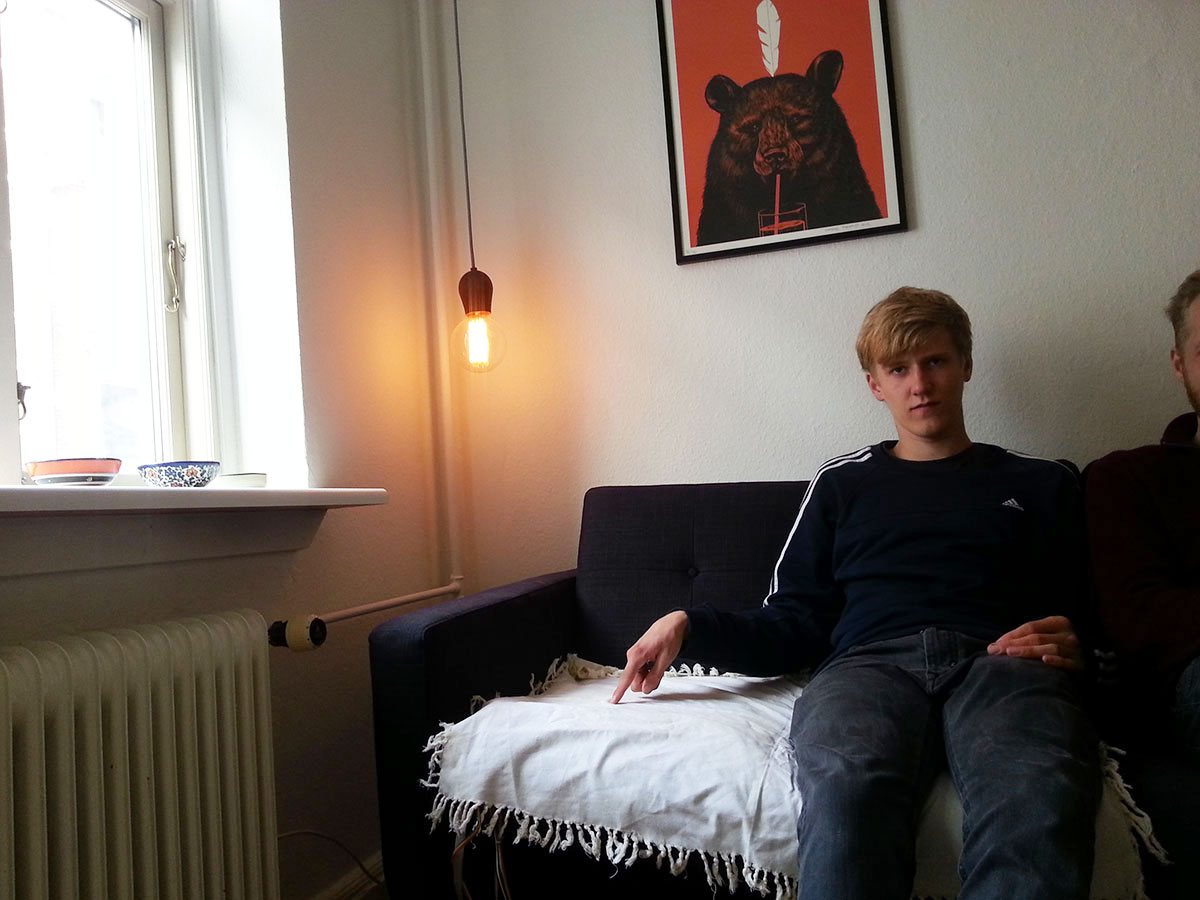
\includegraphics[width=\textwidth]{figures/touch/evaluation/sebastian/sofa_infront_seb}
        \caption{Teenager trying the prototype.}
        \label{fig:textiletouch:eval:sebastian:sofa_front}
    \end{subfigure}%
    \hspace{0.02\textwidth}
    \begin{subfigure}[t]{0.44\textwidth}
        \centering
        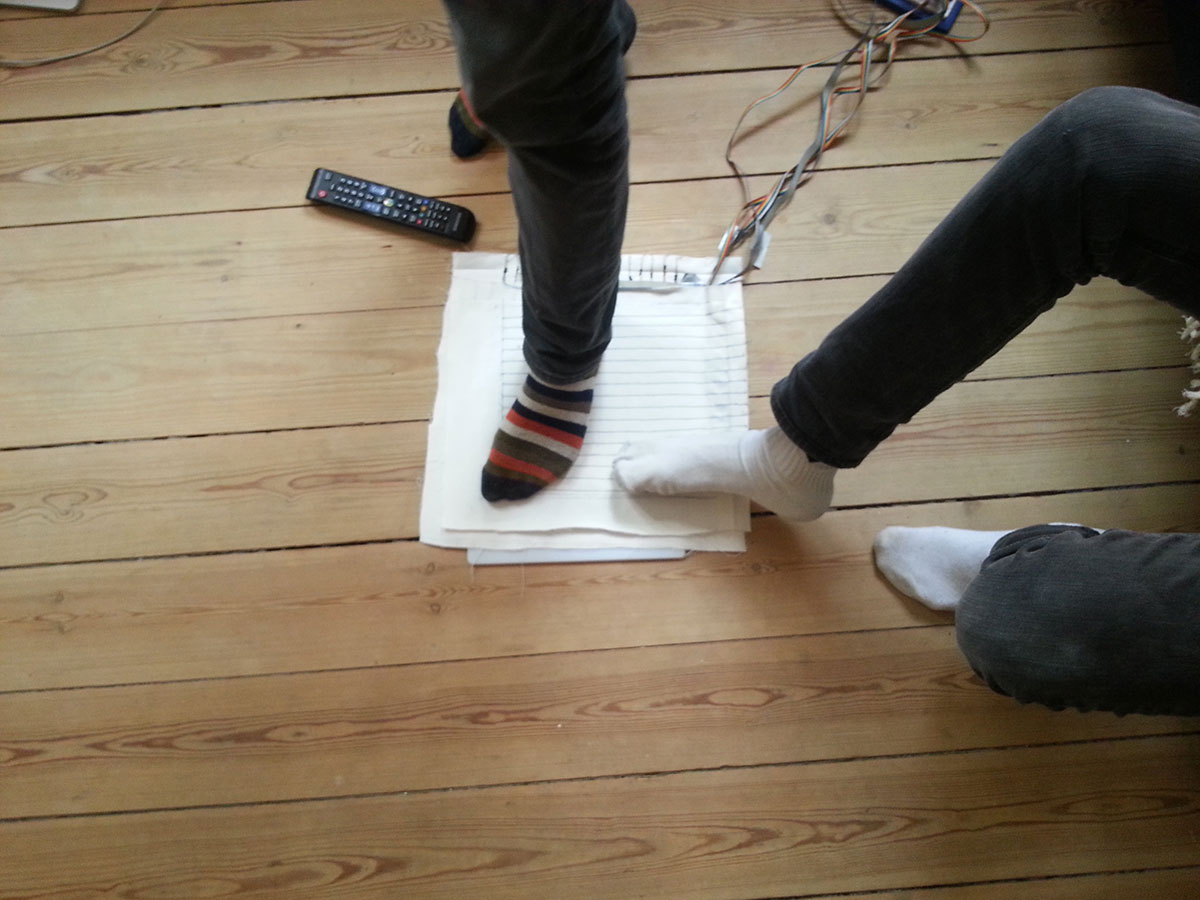
\includegraphics[width=\textwidth]{figures/touch/evaluation/sebastian/feet}
        \caption{Testing foot input on the floor.}
        \label{fig:textiletouch:eval:sebastian:feet}
    \end{subfigure}
    \caption{An selection of photos from an evaluation with a young teenager.}
    \label{fig:textiletouch:eval:sebastian}
\end{figure}

One participant pointed out that he at home considers his TV remote as an ``extension of his arm'' meaning that he can use it and push the right buttons without having to pay visual attention to it. 
After playing around with the prototype and the audio/video application for a while he \emph{mentioned} that he could imagine this kind of touch interaction be even more intuitive as ``the remote is in a sense always at the tip of my finger'' after which he commented that his finger doesn't normally disappear.
\blank
A general concern regarding the use of gestures is that care must be taken when designing interactions based on gestures.
As brought up by several participants, they do not want the complexity of having to learn a completely new interaction language.
In our setup the amount of gesture-based functions implemented was less than 10 which meant that the participants had little or no difficulty in remembering the specific gestures, but in a more complex system problems would definitely arise.
Our chosen gestures were quite simple (lines, crosses, arrows, etc) and functions in the audio and the video application used the same set of gestures for similar functions, easing the shift between the two.
Examples hereof are volume control and a function such as \emph{skip forward} in the audio application that was gesture-wise the same as \emph{channel forward} in the video application.

Another initiative that could lower the learning curve of such a system is to base gestures on the familiarity from other devices such as smart phones, tablets and touchpads.
A lot of people are familiar with gestures such as swipe, pinch, and two-finger scrolls from other devices but as the dollar family of recognisers do not handle real-time interpretation of gestures we have not gone further with this.

\subsection{Potentials of alternative usages}

The ideas for alternative usages were in general very different from the idea of controlling existing devices.
The ideas were more characterised by sensor data being used in situations where meaning is open to interpretation as opposed to a one-to-one mapping between input gesture and function.
For example, several ideas concerning safety and security were discussed.

% toddlers
Parents of toddlers often have floor mats for their child to lay and play on (see figure~\ref{fig:textiletouch:eval:softtiles}).
Instead of having parents checking up on their child every two minutes these mats could have touch fields embedded.
The sensor data can then be abstracted to inform parents about the activity of their child by recording pressure and movement, giving the concerned parent room to do less frequent check ups.
This is actually a very simple setup that does not require a high resolution of the sensor grid and the output required could be condensed to simple states such as, whether the toddler is on the mat and the level of movement activity.

\begin{figure}[h]
  \centering
  \begin{minipage}[b]{.8\textwidth}
    \centering
    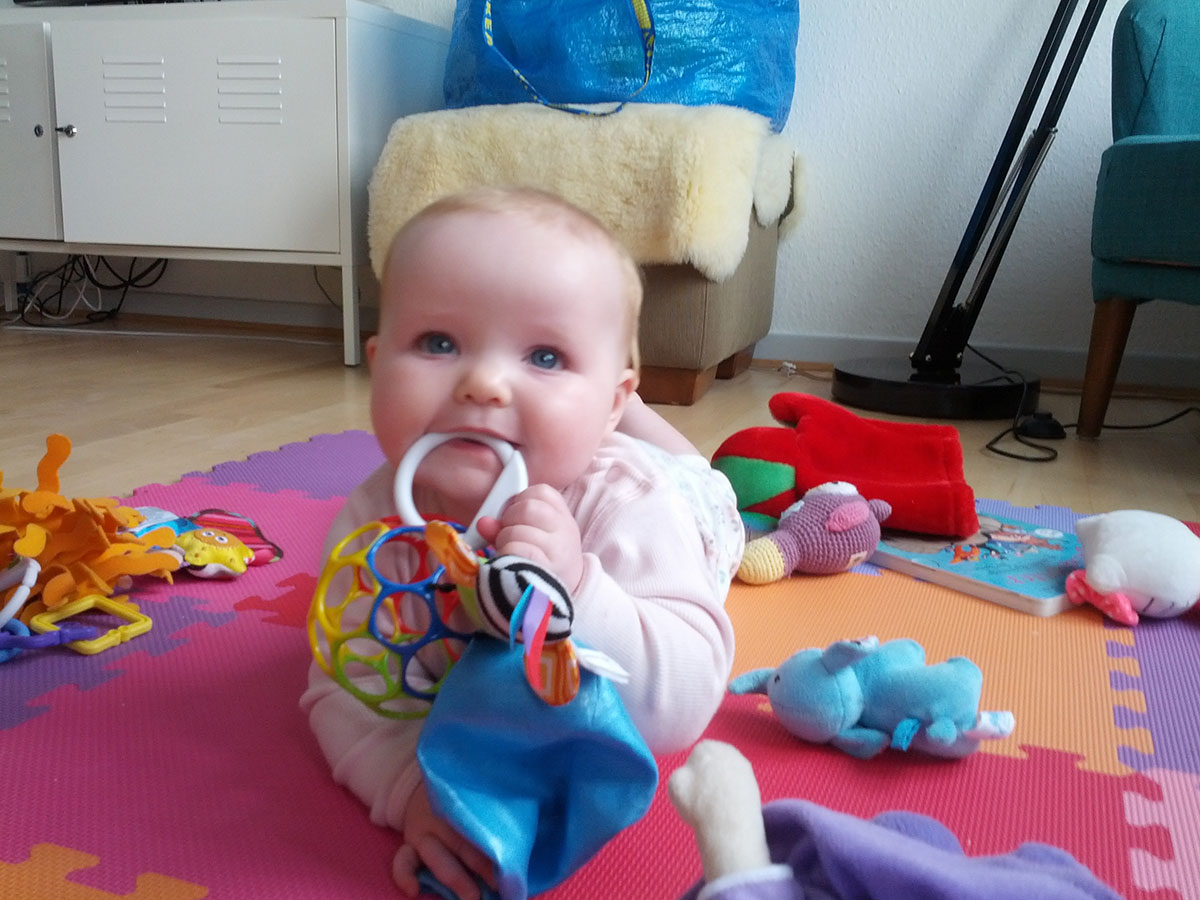
\includegraphics[width=.7\linewidth]{figures/touch/evaluation/softtiles}
  \caption[Toddler on a foam floor mat with puzzle-like tiles for extensibility.]
  {Toddler on a foam floor mat.}
  \label{fig:textiletouch:eval:softtiles}
  \end{minipage}
\end{figure}

% elders
Elderly people with limited physical abilities or people with Parkinson's disease have a tendency to fall over easily.
One of the approaches in reducing the consequences of a fall is to give the elders assistive devices such as wearable fall detectors which can automatically release an alarm in the event of a fall.
An alternative approach, which does not require body equipment, could be to prepare the home with impact sensitive floors or carpets.
Some may base their sense of security in a physical wearable device while others find it inconvenient, a source of irritation, or maybe even an exceedance of personal privacy. 
With safety measurements invisibly integrated into the home the sense of security may be directed towards the scope of the home as a whole.

% Home security
During the evaluations we also discussed a scenario of home security regarding the front door of ones home.
In this scenario we imagined a blank door with no handle and no lock and thereby no need for a key.
Instead the door had an embedded grid of pressure sensors.
We came up with and enacted two different interaction styles for opening the door.
One was a variant of the pattern lock found in many Android smart phones where a set of points must be touched in the correct sequence in order for the door to unlock, see figure \todo{billede af Kaia og Gitte ved doeren 1}.
The other was based on the fact that people have unique signatures which could be used for authentication.
A person would then have to makes strokes (the signature) on the door facade to be authenticated and have the door unlock and open, see figure \todo{billede af Kaia og Gitte ved doeren 2}.

This is a good example of an ad hoc interface \emph{through invisible interfaces embedded into the physical environment}.
Knowledge of the system is a prerequisite to enter in that you are faced with a blank facade with no direct indication of how to enter.
It also confronts the raised issue of invisible interfaces and affordances by using it as an advantage in a security setting where the absence of a lock and door handle would inhibit a trespasser.
\blank
% Sleep cycle
Moving away from the topic of safety and security to the topic of self-tracking, a movement that has gained a lot of popularity in recent years with the advent of consumer gadgets, such as Fitbit\footnote{http://www.fitbit.com/}, Nike+\footnote{http://nikeplus.nike.com/plus/} and loads more. 
These gadgets let you sense just about anything concerning your body, quantifying yourself in numbers.
An example of this is sleep monitoring and optimisation, which in its simplest form only requires a smart phone next to your body in bed, but can take on more advanced forms as well with a variety of body sensors.
With a smart phone the approach is to use the built-in accelerometer to detect movement during sleep to graph the total sleep and derive whether the person is in deep sleep or light sleep.
These data can also be used to trigger the wake-up alarm at moments of light sleep within a specified time frame close to the set alarm time.

A product with the capabilities of our textile touch prototype which can infer the same kind of information by the means of a pressure measurements over time, would be an interesting alternative.
Being integrated as part of a madras or a bed sheet it would be unnoticeable for a sleeping person and would not require a smart phone next to the pillow which some may be precautious about.

This application does not really fall under the category of AHIs, but it is mentioned here for the potential of a discrete and unobtrusive product as a continuation of the self-tracking movement.

\section{Conclusions and future work for Textile Touch}
\label{ch:textiletouch:futurework}

In this chapter we have explored the second of three approaches to constructing ad hoc user interfaces, namely

\begin{quotation}
  \emph{2. Through invisible interfaces embedded into the physical environment.}
\end{quotation}

This exploration has resulted in the prototype Textile Touch which is a textile-based generic touch surface.
Textile Touch was constructed to be embedded into the surfaces of the home environment to enhance it with a digital layer for interaction.
To explore more advanced touch interactions the prototype was programmed to recognise various gestures which we exemplified in a scenario of controlling existing devices of the home.
These gestures are then mapped to control specific functions of an implemented audio/video application as a real-world scenario.

We do not consider Textile Touch as a final prototype but more an explorative prototype which should be used to explore and reveal potential applications and use-contexts.
These potentials have been addressed during three evaluations where both our test application and alternative activities have been discussed.
The evaluations have shown that the prototype worked well enough to test the interaction in a real setting, and it lived up to the expectations as to explore and augment the design space for a generative user evaluation, though with constraints regarding the evaluation of the user experience. 
Furthermore, the evaluations pointed to several diverse alternative applications where the textile touch technology could be utilised, some of which exhibit ad hoc characteristics.

There are several points about the prototype that are candidates for future work.
On the technical side we have already touched upon areas that could benefit from improvement.
Introducing multi-touch would greatly improve the user experience with a richer interaction style compared to that of single-touch.
Combining multi-touch with a more real-time based gesture framework would also allow for a more familiar interaction style as pointed out in the evaluation.
Lastly, feedback through vibrations as a response to touch movements was positively received but the strength and thereby quality of it should very much be improved.